\documentclass[aps,letterpaper,11pt]{revtex4}

\usepackage{graphicx}
\usepackage{float}
\usepackage{verbatim}
\usepackage{amsmath}
\usepackage{amssymb}

\newcommand{\labno}{4}
\newcommand{\labtitle}{Reenacting the Tale of William Tell Using Projectile Motion}
\newcommand{\authorname}{Kevin Truong}
\newcommand{\professor}{Dr. Melanie Lutz}
\newcommand{\classno}{Physics 006}
\newcommand{\labpartners}{Sean Casey, Kevin Castillo, Dulce Payan, and Muhammad Eminic}
\newcommand{\submitdate}{February 21,2017}

\begin{document}

\begin{titlepage}
\begin{center}
\hspace{-136mm}\boxed{{\Large \textsc{Lab No. \labno}}}\\\vspace{30mm}
{\Large \textsc{\labtitle} \\ \vspace{4pt}}
\rule[13pt]{\textwidth}{1pt}\\ \vspace{150pt}
{\large By: \authorname \\ \vspace{10pt}}
Lab Partners: \labpartners \\
Instructor: \professor \vspace{10pt} \\
Solano Community College\\ \classno \\ \vspace{10pt}
\submitdate
\end{center}
\end{titlepage}

\section{Abstract}

 Being able to shoot an apple of a child's head is a tall task, especially when an arrow is heavily affected by air resistance. In this experiment, a marble was used instead of an arrow to shoot at the "child's" head. Using kinematic equations and collected data it was possible to calculate the average initial velocity of the marble launched, 3.1411$\frac{m}{s}$. The angle that was given during the experiment was $52^o$, and the final calculated distance that the child needed to be placed was .6589953m which seemed reasonable. However, the result of the lab was we shot the child in the face with the marble and knocked his head off. 

\section{Introduction}

Determining the motion of a projectile at a certain angle to hit a specific point is possible using the kinematic equation  $x = x_0+v_{0x}t+\frac{1}{2}a_xt^2$ and $y = y_0+v_{0y}t+\frac{1}{2}a_yt^2$ where the equation for x affects the horiztonal(x) direction and the equation for y affects the vertical(y) direction. The only thing that needs to be noted is that the time that it takes the projectile to hit the specific point is equal in the x and y direction, to be able to eliminate time from the equation. Using these kinematic equations in tandem, it is possible to calculate any motion made by the projectile, given sufficient amount of information. 

\section{Experimental Details}

Equipment for this experiment includes a computer, a launcher, a marble, some white copy paper, some carbon paper, a meter stick, Microsoft Excel, and child and apple. The computer was used as a way to input and save all of the data that was collected throughout the lab. The launcher was clamped level with the table, so that the origin of our axis would be the table; it was possible to change the angle of the launcher to test out how the angle would change the launch of the marble. The launcher also had two force settings: One notch which was the analogue of low on the cart, and the deeper-second notch which was the analogue of high on the cart. The launcher was "fired" by pulling a string at the end of the launcher, it is important to have the same person launch the launcher throughout the lab to try to keep the scenerios as uniform as possible. The marble was used as the ammunition for the launcher to shoot, the marble was being shot at the "apple." The white paper was used in tandem with the carbon paper to trace where the marbles would land along the table, once it was shot. The meter stick was used to measure the distance from the edge of the table to the location that the marble had landed, so the data would be inputted into the computer. Microsoft Excel was used to input all of the data and create the graphs that would represents the data collected, the data that was collected was the distances that the marble landed after it was launched at a certain angle and at a certain force. The child and apple were used to test the calculations, to see if the calculations were incorrect and the apple would be shot of the child's head or if the child was going to die. 

Data was collected at both notches of force and between the angles of twenty and seventy with five degree intervals. This data was collected to analyze how accurate the launcher was and to use Excel to calculate the initial velocity once the marble was launched out of the launcher. The marble was launched twice at each interval and at each notch of force to make sure the data collected was correct. The initial velocity was calculated by using the linear regression of the velocity vs. time graph.  

\vspace{-10mm}

\subsection{The Diagram of the Setup to Shoot the Apple}

\begin{center}
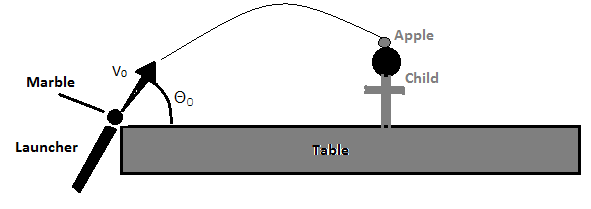
\includegraphics[width=4in]{Setup.png}
\end{center}

\section{Procedures, Results and Analysis}

\subsection{Determining $v_0$ as a function of $\theta_0$}

To obtain the value of $v_0$, it's necessary to collect data on the distance that the marble travels when the angle is changed when using the same initial force. It's important to note that there was some horizontal distance from the opening of the launcher to the edge of the table, so it's necessary to add the distance between the opening of the launcher and the edge of the table to the measured range of the marble launch. The distance from the opening of the launcher and the edge of the table was 0.04m.  It was decided to use one notch as the force that the marble will be launched at because during the experiment the first notch produced a more consistent set of data. The marble was launched at each setting of force twice and the first notch's range was very close on each launch. While second notch was sometimes close and sometimes quite far apart. The marble launcher was set to angles between twenty and seventy degrees with five degree increments, so there was a total of eleven angels that had data collected from, that being 20, 25, 30, 35, 40, 45, 50, 55, 60, 65, and 70.   

\subsubsection{Setup for Measuring the Initial Velocity as a function of the Initial Launch Angle}

\begin{center}
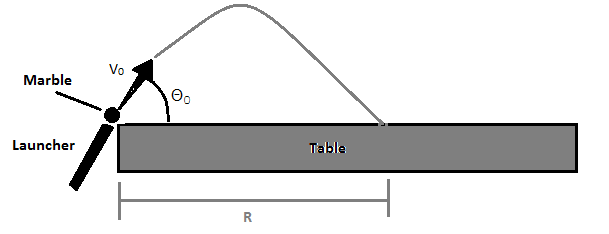
\includegraphics[width=4in]{FindingVNaught.png}
\end{center}

The diagram directly above models the setup that was used to obtain range values at certain angles, so these collected data could be placed into Excel. With the collected range values and the corresponding angles, it was possible to calculate $v_0$ by using the equation: (Actual derivation in Appendices)

$$ v_0=\sqrt[2]{\frac{gR}{2sin(\theta)cos(\theta)}}$$ 


where g was 9.8$\frac{m}{s^2}$, R was the horizontal distance that the marble traveled, and $\theta$ was the initial angle that the launcher was set at. However, Excel only calculates in radians so it was necessary to change the angles to radians using the equation:

$$ Radians = \frac{\pi}{180^o}*degrees$$  

The data table below is the range that the marble traveled at each angle, as the launcher was set at the first notch of force. The initial velocities in the third column was calculated using the equation above the equation to calculate radians to solve for $v_0$. 

\begin{center}
\underline{Data Table}\\
\vspace{5mm}
\begin{tabular}{ |c|c|c| }
\hline
Angle & Range(m) & Initial Velocity($\frac{m}{s})$\\
\hline
20 & 0.657 & 3.164914443\\
\hline
25 & 0.755 & 3.107846285\\
\hline
30 & 0.868 & 3.134062006\\
\hline
35 & 0.928 & 3.110957784 \\
\hline
40 & 0.973 & 3.111671402\\
\hline
45 & 0.975 & 3.091116303\\
\hline
50 & 0.962 & 3.094032309\\
\hline
55 & 0.917 & 3.092465031\\
\hline
60 & 0.845 & 3.092260526\\
\hline
65 & 0.760 & 3.118120185\\
\hline
70 & 0.640 & 3.123699704\\
\hline
\end{tabular}
\end{center}

In Excel column A was dedicated to the angles that the marble was being shot at. Column B was dedicated to the total distance (distance from the opening of the launcher to the marble's landing point). Column D was the converted radians from the angles used. Column E was the angles again, so it was easy to create the velocity vs. angle graph in Excel. Column F was dedicated to the initial velocities that were calculated. From this data, it was possible to create a Range vs. Angle and Velocity vs. Angle graphs. On both of these graphs there is a title, axis titles, caption, and data points. The velocity vs. angle graph had a linear regression that was used to obtain the average initial velocity to be used in the final calculations. Figure 1 is the Range Vs. Angle graph that was created using the collected data, it has a parabolic shape with 45 degrees as the maximum range. Figure 2 is the Velocity Vs. Angle graph that has a fairly straight linear regression.

\begin{center}
\vspace{-20mm}
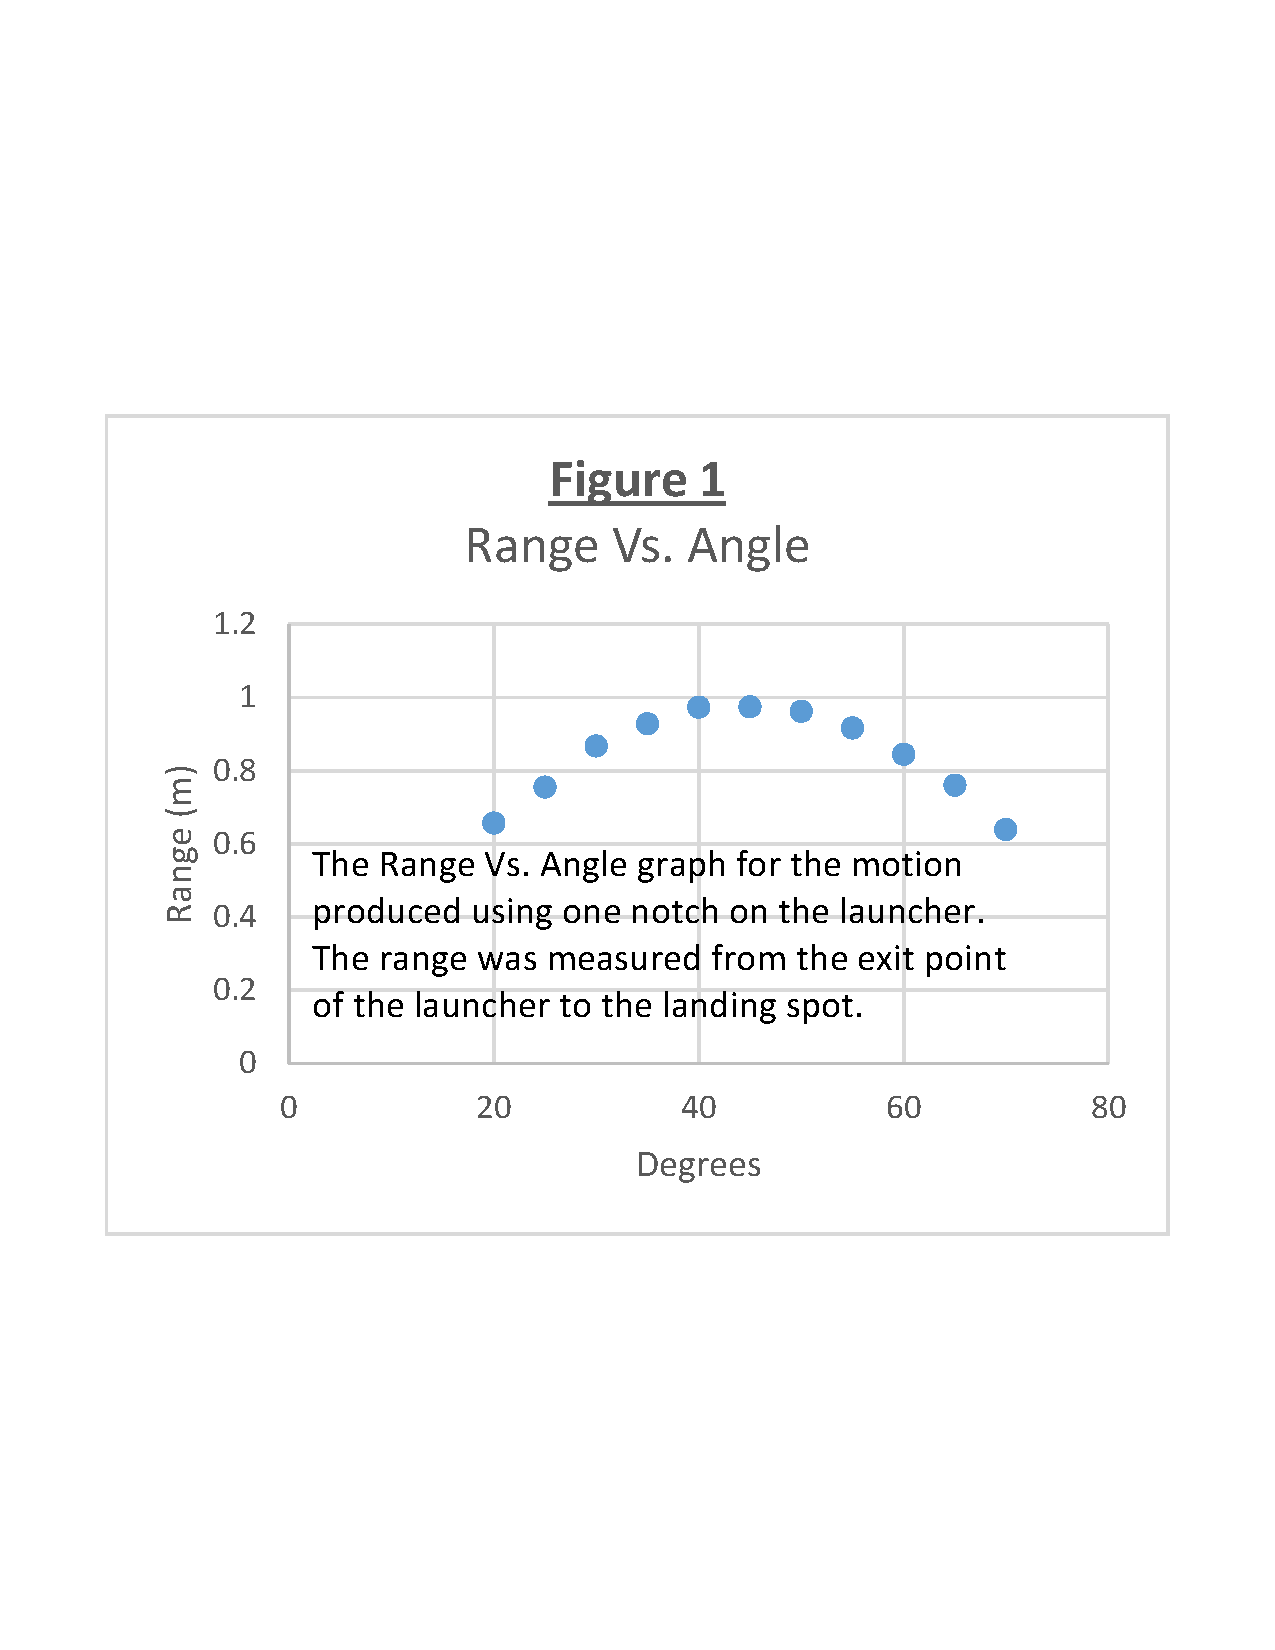
\includegraphics[width=4in]{RangeVsAngle.pdf}\\
\vspace{-50mm}
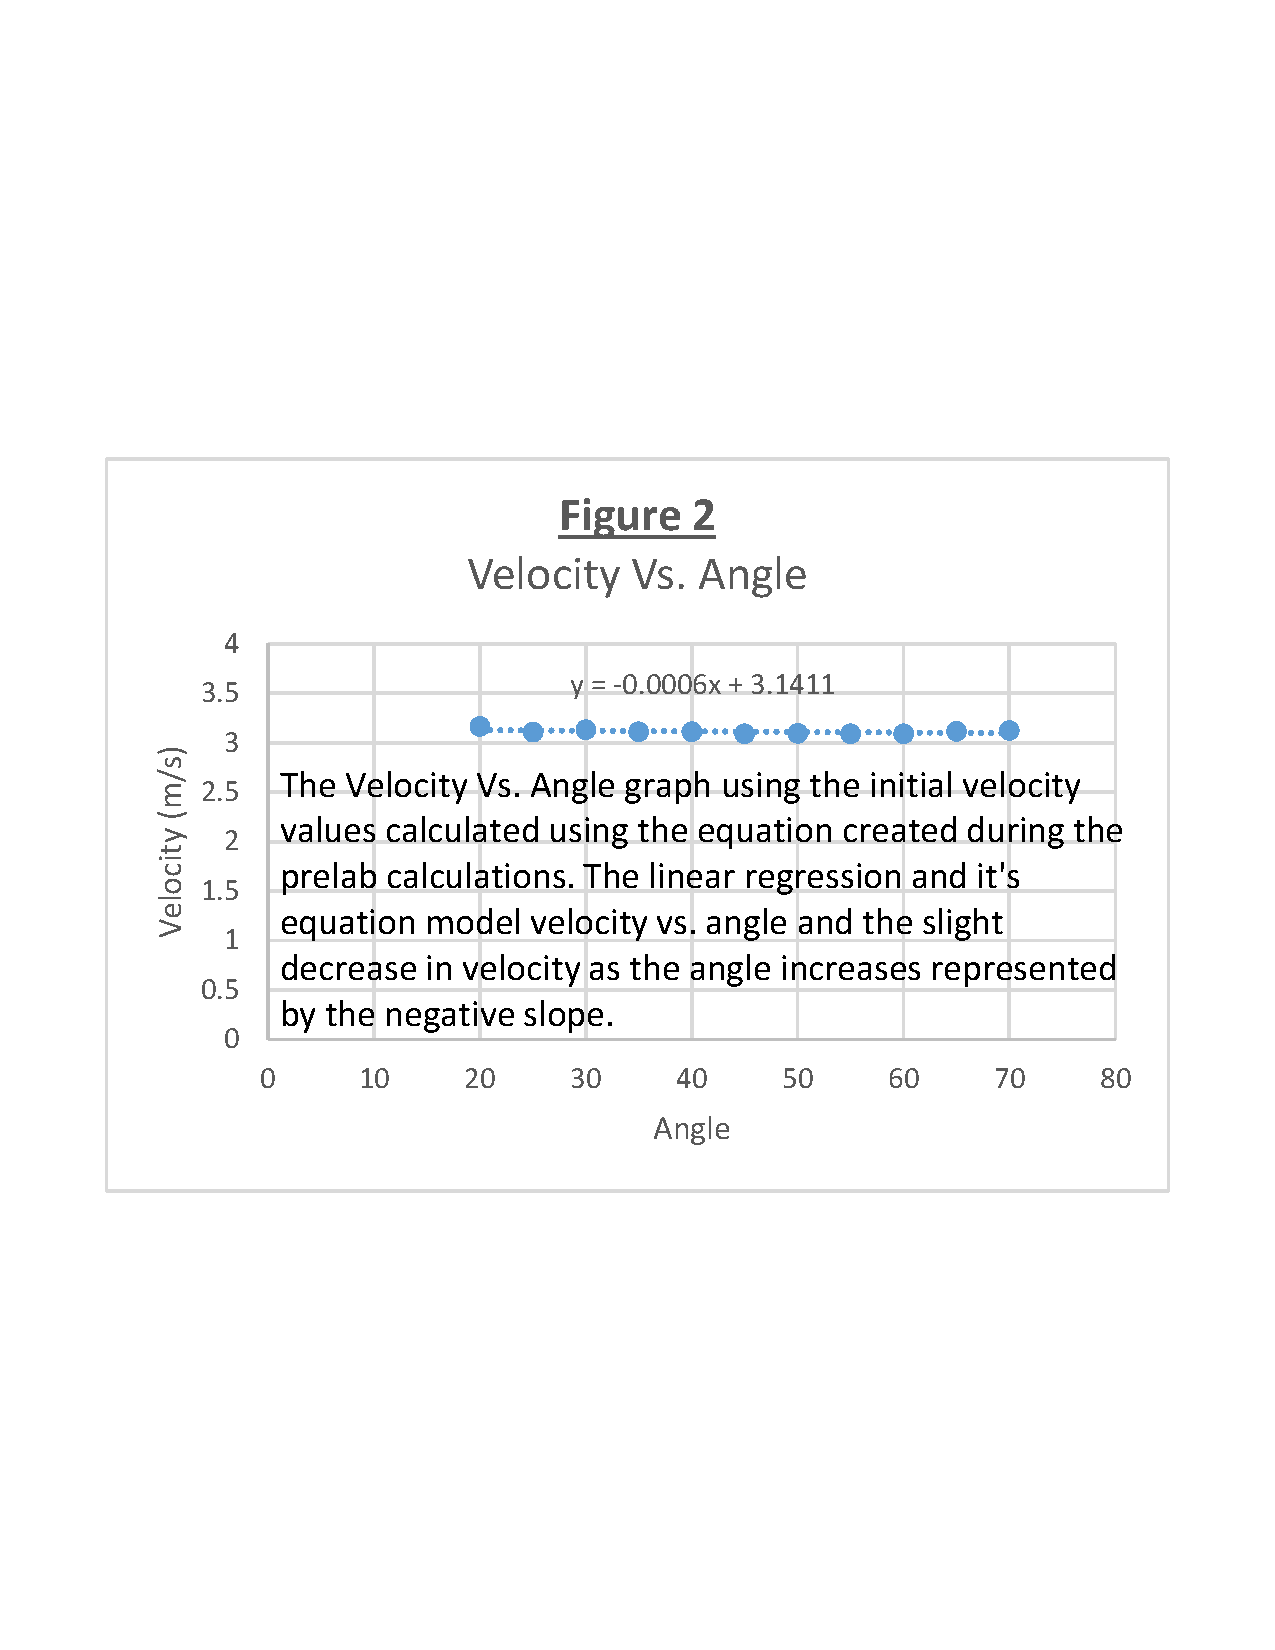
\includegraphics[width=4in]{VelocityVsAngle.pdf}
\end{center}

\newpage

The linear regression on the velocity vs. angle graph had an equation of:

$$ v_0=-0.0006\theta+3.1411$$ 

This equation shows that the average initial velocity was 3.1411 and the slope of the equation was -0.0006. The slope explains that as the angle increases the initial velocity decreases, and this can be attributed to gravity; as the angle increases the marble's initial velocity is affected, more, by gravity. 

\subsection{Preparing for the Shot}

 Now that the average initial velocity was obtained in part A, it's possible to calculate the distance away the child has to be placed to shoot the apple with the equation (the derivation for this equation with be in the appendices):
 
 $$ x=\frac{(v_0cos(\theta_0))^2}{g}[tan(\theta)\pm\sqrt[2]{tan^2(\theta_0)-\frac{2gy}{(v_0cos(\theta_0))^2}}]$$
 
 Since the target is to hit the marble on the way down from the launch, the value that will be used will be the greater value of the two calculated values using the equation above. $v_0$ is the average initial velocity that was obtained in the first section, $\theta_0$ is the initial angle that will be given during the lab, g is gravity, and y is the height of the apple from the table. The equation already accounts for the negative value of gravity, so the value that is substituted for g will be 9.8$\frac{m}{s^2}$. 
 
 \section{The Moment of Truth}
 
 The angle that was given was $52^o$. $v_0$ from section A was 3.1099$\frac{m}{s}$. The height from the table to middle of the marble(apple) was .263m, so this will be the y value in the equation. Replacing all of the givens into the equation:
 
$$ x=\frac{((3.1099\frac{m}{s})cos(52^o))^2}{9.8\frac{m}{s^2}}[tan(52^o)\pm\sqrt[2]{tan^2(52^o)-\frac{2(9.8\frac{m}{s^2})(.263m)}{((3.1099\frac{m}{s})cos(52^o))^2}}]$$

\[ x \approx 0.2985755m,\hspace{1mm} 0.6589953m\]

The first x value is when the marble reaches that height when traveling upward, the second x value is when the marble reaches that height traveling downward. Since the experiment wants the x value of the marble going downward, the x value that was used was \boxed{0.6589953m}. It should be noted that this distance will be from the opening of the launcher to the child. 

However, after all of the calculations the experiment was a failure because we did not manage to hit the marble off the child's head. Instead we shot the child in the face, twice. The cause of this failure was due to incorrect measurements, I don't believe that the measurements started at the opening of the launcher, and instead the measurements began at the edge of the table which caused the child too be too far away from the correct position. 

\section{Discussion} 

 When deriving the distance to place the child, there was two values because the quadratic equation was used. However, the apple had to be hit on the way down from the launch, the greater value of x was used. The smaller value was the marble going upward from the launch and reaching the specific height of the child. 
 
 Even though, our group didn't shoot the apple off the child's head; this experiment could have been substantially more difficult if air resistance had a bigger role, for example if an arrow was shot instead of a round marble. If we had measured the distance correclty from the exit of the launcher, we would have hit the marble(apple) off the child's head.

\section{Appendices}

\underline{Initial Velocity Derivation}

If we place the origin at the opening of the launcher, it makes the derivation easier.\\

\begin{center}
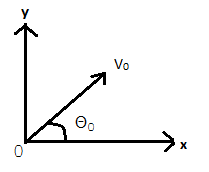
\includegraphics[width=2in]{VNAUGHTGRAPH.png}

Note: $tan(\theta_0) = \frac{v_{0y}}{v_{0x}}$ and $v_{0x}=v_0cos(\theta_0)$ using geometry

\end{center}

The important thing to note is that the time that the marble travels to reach the landing location is equal in the x and y direction. Therefore, we can solve for t in terms of x and then direct substitute it into t for the equation in the y direction. First using the equation:

\[ x = x_0+v_{0x}t+\frac{1}{2}a_xt^2\]

since $x_0=0$ because the marble begins at the origin, and $a_x=0$ because there is no force accelerating the marble in the x direction. The equation can be reduced to:

$$ x=v_{0x}t$$

solving for t:

$$ t=\frac{x}{v_{0x}}$$

and then using the equation in the y direction:

\[ y = y_0+v_{0y}t+\frac{1}{2}a_yt^2\]

plug in t in terms of x:

\[ y = y_0+v_{0y}(\frac{x}{v_{0x}})+\frac{1}{2}a_y(\frac{x}{v_{0x}})^2\]

from the note above, we know that $tan(\theta_0) = \frac{v_{0y}}{v_{0x}}$ and $v_{0x}=v_0cos(\theta_0)$. Again since the marble is starting at the origin $y_0=0$. Since the landing location is exactly the same height as the origin, $y=0$ as well. The acceleration that is affecting the marble is gravity once it's in the air, and gravity works in the y direction, in this case. Therefore $a_y=-g$, it's negative because gravity works downward in respect to the origin that we decided. 

The equation can be simplified to:

\[ 0=0+xtan(\theta_0)-\frac{g}{2}(\frac{x}{v_0cos(\theta_0)})^2\]

with simple arithmetic, we can solve for $v_0$:

\[ \boxed{v_0=\sqrt[2]{\frac{gR}{2sin(\theta_0)cos(\theta_0)}}}\]

$x=R$ because x is just the range that marble travels.

\underline{Distance away from the launcher to place the child}

\begin{center}
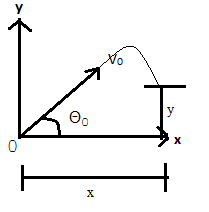
\includegraphics[width=2in]{FINALCALC.png}\\
Note: $tan(\theta_0) = \frac{v_{0y}}{v_{0x}}$ and $v_{0x}=v_0cos(\theta_0)$ using geometry
\end{center}

Again the important thing to note is the time that the marble takes to hit the apple will be the same in the x and y direction. Therefore, we will solve for t in terms of x and then plug in t for the equation in the y direction and then solve for x. First we will use the equation:

\[ x = x_0+v_{0x}t+\frac{1}{2}a_xt^2\]

since $x_0=0$ because the marble begins at the origin, and $a_x=0$ because there is no force accelerating the marble in the x direction. The equation can be reduced to:

$$ x=v_{0x}t$$

solving for t:

$$ t=\frac{x}{v_{0x}}$$

and then using the equation in the y direction:

\[ y = y_0+v_{0y}t+\frac{1}{2}a_yt^2\]

plug in t in terms of x:

\[ y = y_0+v_{0y}(\frac{x}{v_{0x}})+\frac{1}{2}a_y(\frac{x}{v_{0x}})^2\]

from the note above, we know that $tan(\theta_0) = \frac{v_{0y}}{v_{0x}}$ and $v_{0x}=v_0cos(\theta_0)$. Again since the marble is starting at the origin $y_0=0$. Since the landing location is going to be the height from the table to middle of the marble(apple), we can keep y as y. The acceleration that is affecting the marble is gravity once it's in the air, and gravity works in the y direction, in this case. Therefore $a_y=-g$, it's negative because gravity works downward in respect to the origin that we decided. 

The equation can be simplified to:

\[ y=0+xtan(\theta_0)-\frac{g}{2}(\frac{x}{v_0cos(\theta_0)})^2\]

Getting all of the variables onto one side, we obtain a quadratic:

\[ (\frac{g}{2(v_0cos(\theta_0))^2})x^2-tan(\theta_0)x+y=0\]

We can then use the quadratic formula to solve for the values of x:

\[ x=\frac{tan(\theta_0)\pm\sqrt[2]{tan^2(\theta_0)-4(\frac{g}{2(v_0cos(\theta_0))^2})(y})}{2(\frac{g}{2(v_0cos(\theta_0))^2})}\]

Using arithemetic, the equation can be simplified to:

\[ \boxed{x=\frac{(v_0cos(\theta_0))^2}{g}[tan(\theta_0)\pm\sqrt[2]{tan^2(\theta_0)-\frac{2gy}{(v_0cos(\theta_0))^2}}]}\]


\section{References}

\hspace{-6.5mm}
Projectile Motion Physics 06 Lab, Dr. Melanie Lutz\\



\end{document}
